\documentclass{standalone}

\usepackage{TikzStyle}
\usepackage{mystyle}

\begin{document}
    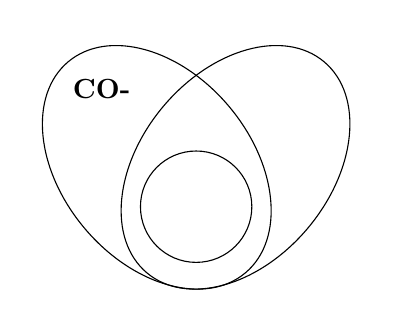
\begin{tikzpicture}
        \node[draw,circle,inner sep=0.5cm] () at (0,0) {$\PClass$};
        \draw (0.5,0.5) ellipse [x radius=1.2cm,y radius=1.75cm,rotate=-40];
        \draw (-0.5,0.5) ellipse [x radius=1.2cm,y radius=1.75cm,rotate=40];
        \node () at (-1.2,1.5) {$\textbf{CO-}\NPClass$};
        \node () at (1.5,1.5) {$\NPClass$};
    \end{tikzpicture}
\end{document}
